\chapter{Development} \label{chap:desenv}

In this section, we describe the development of the \textit{zCart} smart cart
prototype. All the source code related to the prototype is available at a
GitHub repository\footnote{https://github.com/fsmiamoto/zcart}

\section{Design}
\label{sec:design}

As a first step in developing our prototype, a set of
high level goals was defined to guide the initial technical design:

\begin{enumerate}
    \item Handle user interactions and give visual feedback
    \item Store the current set of products present in the cart and their respective information
    \item Recognize the addition or removal of products, including quantities.
\end{enumerate}

With those goals in mind, the high level architecture of the prototype
was designed and is shown in Figure \ref{fig:architecture}.

For each goal, a dedicated software application will be used and those
applications will communicate using \siglaPt{TCP}{Transmission Control Protocol}
network sockets \cite{Kurose2013} with industry standard application protocols such as
\siglaPt{HTTP}{Hypertext Transfer Protocol}\footnote{First defined in
\siglaPt{RFC}{Request For Comments} 1945} and WebSocket\footnote{Defined in RFC 6455}.
Most of the HTTP communication will follow the widespread REST pattern \cite{Roy2000}.

\begin{figure}[H]
	\centering
	\caption[High level architecture of zCart]{High level architecture of zCart}
    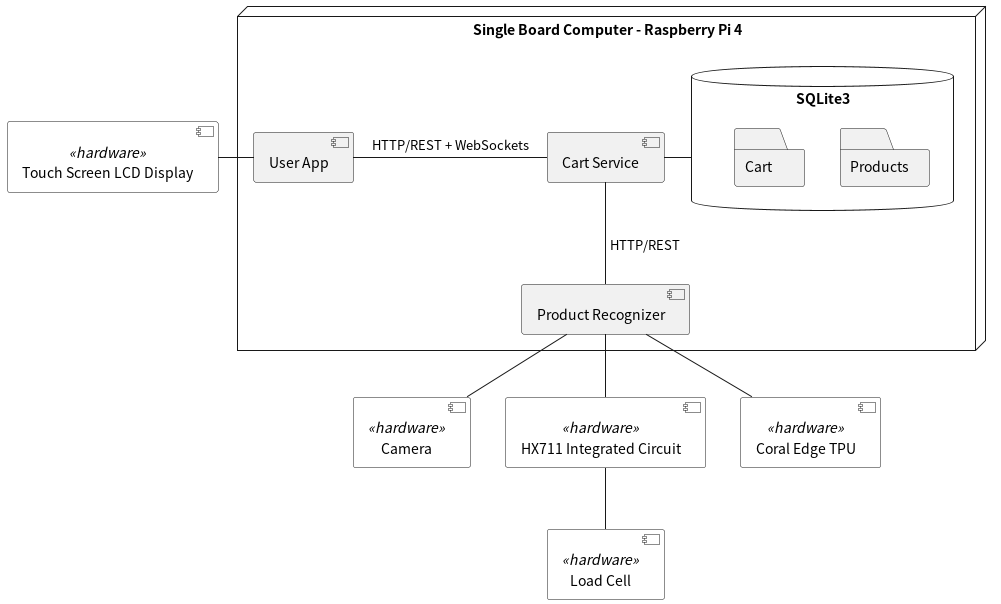
\includegraphics[width=1\textwidth]{./images/zCart.png}
	\fonte{}
	\label{fig:architecture}
\end{figure}

For handling the first goal, the \textit{User App} will request data
from other applications and will display the information to end users and allow
them to interact with the cart using a touch enabled LCD display. 

The \textit{Cart Service} will be in charge of the second goal,
handling requests from the \textit{User App}, which asks for data 
on the products that are detected and notifies the completion of a purchase order 
when the user completes the checkout. The \textit{Cart Service} uses a
\textbf{relational database} \cite{Silberschatz2010} as its primary database. Namely
\textbf{SQLite}, considered to be the world's most deployed database due to its
massive adoption on mobile
devices\footnote{https://www.sqlite.org/mostdeployed.html}. The simplicity of
SQLite, the entire database is contained within a single file, great
library support on common programming languages and the use of the familiar
relational modeling, including \siglaPt{SQL}{Structured Query Language}
\cite{Nield2016}, were key factors in choosing it.

In order to provide real time updates to the \textit{User App}, the Cart Service has a
WebSocket API endpoint that allows the User App to listen to updates such as a product addition
and then display a notification to the end user.

For the third goal, the \textit{Product Recognizer} application will be responsible
for processing a camera feed and weight sensor data to be able to tell if any products
were added of removed from the cart. Any detected changes will be communicated to the
Cart Service, which will be responsible for persisting those changes on the database. 

All three applications will execute under a Linux \cite{Tanenbaum2015} 
based environment on a Raspberry Pi\footnote{https://www.raspberrypi.com} 4 Single Board
Computer (\siglaPt{SBC}{Single Board Computer}) - a complete computer built on a single 
circuit board with a microprocessor, memory and input/output devices.

The advantages of using a Linux environment for the development are many, but
being able to leverage its concurrency capabilities, having built-in drivers
for readily available hardware and leveraging open source projects are some 
worth mentioning.

An End-to-End sequence diagram of an example action is shown in Figure \ref{fig:e2eseq}.

\begin{figure}[H]
	\centering
	\caption[End-to-end sequence diagram for a product addition]{End-to-end sequence diagram for a product addition}
    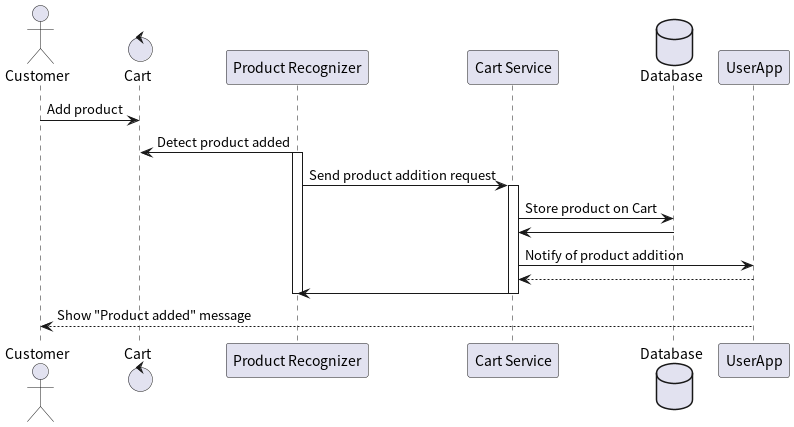
\includegraphics[width=1\textwidth]{./images/E2E.png}
	\fonte{}
	\label{fig:e2eseq}
\end{figure}

\subsection{Architectural Guidelines}
In creating the zCart architecture, the following guidelines were followed:

\begin{itemize}
    \item Create a separate software application for each goal domain
    \item Use well defined standards for communication between applications.
    \item All databases should be owned by a single application. 
    \item Any interaction that requires an update to a given database that is
        not owned by an application should be done through an API and not
        directly on the database.
    \item Decouple the user interface from how the data displayed is stored and transmitted
\end{itemize}

These guideline are based on known best practices from the software 
development industry including API-first design and segregation of
responsibilities \cite{Sam2021,Kong2022}, which are key for future architectural
evolution.

In the next sections, each application will be discussed in further detail.

\section{User App}

For developing the User App, we have used web technologies such 
as HTML, CSS \cite{Duckett2011} and JavaScript \cite{Flanagan2020} using the 
React\footnote{htps://reactjs.org} framework. 

Using web-based technologies allows the User App to be displayed on any 
device capable of running a web browser; and having mature tooling for 
development, testing and debugging are important factors that influenced 
our decision.

As an alternative, developing Linux native graphical applications through
toolkits such as GTK\footnote{https://gtk.org} and Qt\footnote{https://qt.io}
might have yielded better performance but our unfamiliarity with those would be
a challenge.

\begin{figure}[H]
	\centering
	\caption[User App Interface display a single product]{User App Interface displaying a single product}
    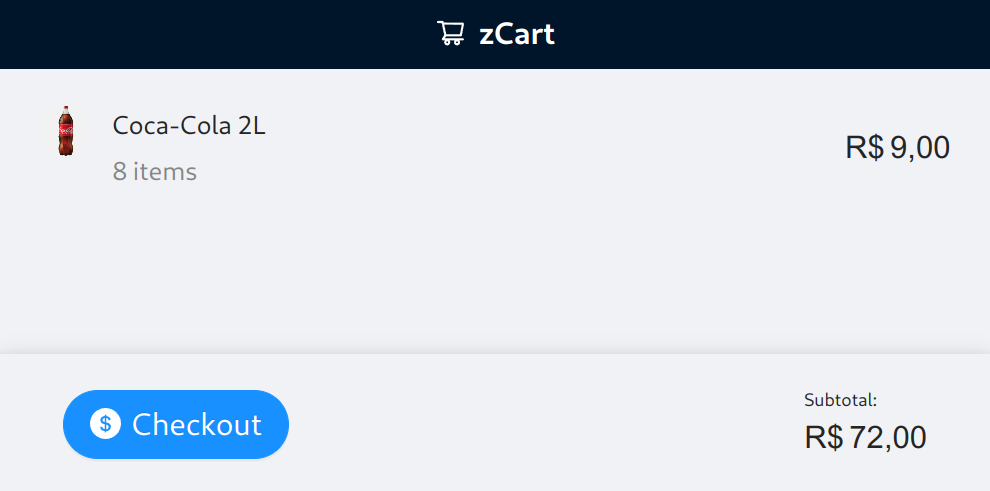
\includegraphics[width=0.8\textwidth]{./images/ui.png}
	\fonte{}
	\label{fig:userapp}
\end{figure}

As shown in Figure \ref{fig:userapp}, the main objective of the User App is to
provide a visual feedback mechanism for end users of the zCart. It displays the
current products added to the cart, their amounts and also the price for each
item. The subtotal price for all products added to the cart is calculated and
also displayed on the interface. Notifications are also displayed when the user
adds or removes a product from the cart. 

Finally, the User App provides a \textit{Checkout} button to simulate the payment process
and act as a Proof-of-Concept (\siglaPt{PoC}{Proof-of-Concept}), since a functional
implementation of a payment mechanism is out of scope for our prototype.

More screenshots showing the user experience are available in Appendix \ref{ap:userapp}.

In terms of the data flow, the User App requests all data from the Cart
Service, which exposes API endpoints for getting the list of products of a
given cart, establishing a WebSocket connection for notifications and
performing the PoC checkout. Figure \ref{fig:userappdataflow} displays the
endpoints of the Cart Service used by User App.

\begin{figure}[H]
	\centering
	\caption[User App and Cart Service interactions]{User App and Cart Service interactions}
    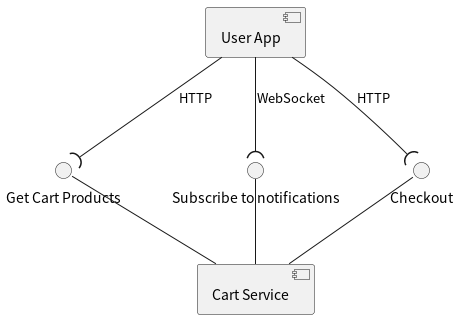
\includegraphics[width=0.6\textwidth]{./images/diagrams/UserApp.png}
	\fonte{}
	\label{fig:userappdataflow}
\end{figure}

\section{Cart Service}

As described in Section \ref{sec:design}, the Cart Service will act as a
centralized storage of the overall \textbf{state} of the cart.

For that, it will responsible for managing the SQLite database and exposing API
endpoints for the required state changes e.g. adding a product, as shown in 
Figure \ref{fig:cartservicearch}.

\begin{figure}[H]
	\centering
    \caption[Cart Service architecture]{Cart Service architecture. The database
    is contained withing the Cart Service boundary and it is not exposed in the
    public APIs}
	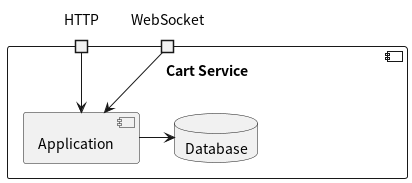
\includegraphics[width=0.6\textwidth]{./images/diagrams/CartService.png}
	\fonte{}
	\label{fig:cartservicearch}
\end{figure}

For the HTTP endpoints, the application uses the REST \cite{Roy2000} pattern
with JavaScript Object Notation (\siglaPt{JSON}{JavaScript Object
Notation})\footnote{https://json.org} as the data-interchange format, both
being widely employed in the software industry. Table \ref{tab:cartendpoints} displays all the API
endpoints created.

\begin{table}[H]
	\centering
    \caption[Cart Service API endpoints]{Cart Service API Endpoints.}
	\begin{tabular}{c | c|c}
		\hline 
        HTTP Method & URI & Description \\
		\hline
        \texttt{GET} & \texttt{/cart/:cartId} & Get the cart data with the product listing \\
        \texttt{POST} & \texttt{/cart/:cartId/products} & Add or remove a product from the cart \\
        \texttt{POST} & \texttt{/cart/:cartId/checkout} & Perform checkout, emptying the cart \\
		\hline 
	\end{tabular}
	\fonte{}
    \label{tab:cartendpoints}
\end{table}

An example response of the \texttt{GET /cart/:cartId} endpoint is shown in
Listing \ref{lst:response}.

\begin{sourcecode}
\caption{Example response for the \texttt{GET /cart/:cartId} endpoint using JSON}
\begin{lstlisting}[label={lst:response}]
{
  "id": "1",
  "products": [
    {
      "cart_id": "1",
      "product_id": "1",
      "quantity": 11,
      "product": {
        "id": "1",
        "name": "Coca Cola",
        "description": null,
        "price": 5.99,
        "image_url": "https://zcart-test-images.s3.amazonaws.com/coca2l.png"
      }
    },
  ]
}
\end{lstlisting}
\fonte{}
\end{sourcecode}

For implementing the Cart Service, the Go\footnote{https://go.dev} programming
language was used alongside the Fiber\footnote{https://gofiber.io/} framework,
which provides great support for the creation of a HTTP Server and also
handling the WebSocket connections.

One of the advantages of the Go language is the use of statically compiled
native binaries, which allows running the application without the need to
install any additional operating system libraries on the Linux environment. 

\section{Product Recognizer}

At the core of the zCart prototype is the Product Recognizer application,
responsible for the product detection based on computer vision and weight
sensing.

For achieving its goal, the Product Recognizer has three main components, as shown in Figure
\ref{fig:productrecognizerarch}.

\begin{figure}[H]
	\centering
	\caption[Product Recognizer Components]{Product Recognizer Components. Detected events will be communicated to the Cart Service for persistence}
    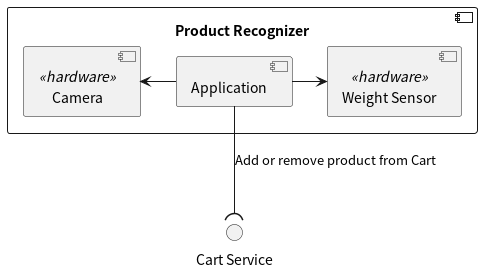
\includegraphics[width=0.6\textwidth]{./images/diagrams/ProductRecognizer.png}
	\fonte{}
	\label{fig:productrecognizerarch}
\end{figure}

Each of these components will be described in more detail in the next subsections.

\subsection{Weight Sensor}

For the Weight Sensor, we've used two main hardware components, shown on Figure \ref{fig:weighttesting}:
\begin{itemize}
    \item  A 10 Kilogram Load Cell
    \item HX711 Integrated Circuit
\end{itemize}

The HX711 is a 24-bit analog-to-digital converter (\siglaPt{ADC}{Analog-to-Digital Converter})
capable of outputting data in a serial interface \cite{Avia2022}.

It has two channels for analog input with channel A having programmable gains of 128 or 64 and
can function using both 3.3V and 5V standard digital voltage levels. The pinout is shown
in Figure \ref{fig:hx711pinout}.

One of its advantages is is that there's no need to program internal registers,
all controls to the chip are through its pins. Additionally, it consumes only
1,5 mA under normal operation and has an on-chip power supply for the connected
load cell, making it a great choice for our prototype.

\begin{figure}[H]
	\centering
	\caption[HX711 Pinout for the SOP-16L package]{HX711 Pinout for the SOP-16L package}
    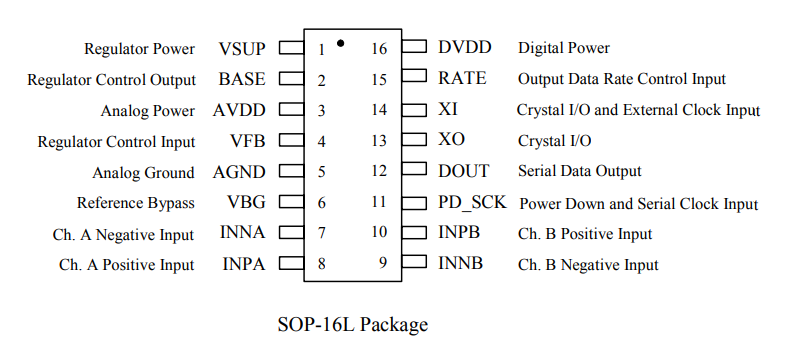
\includegraphics[width=0.9\textwidth]{./images/hx711-pinout.png}
    \fonte{\cite{Avia2022}}
	\label{fig:hx711pinout}
\end{figure}

\begin{figure}[H]
	\centering
	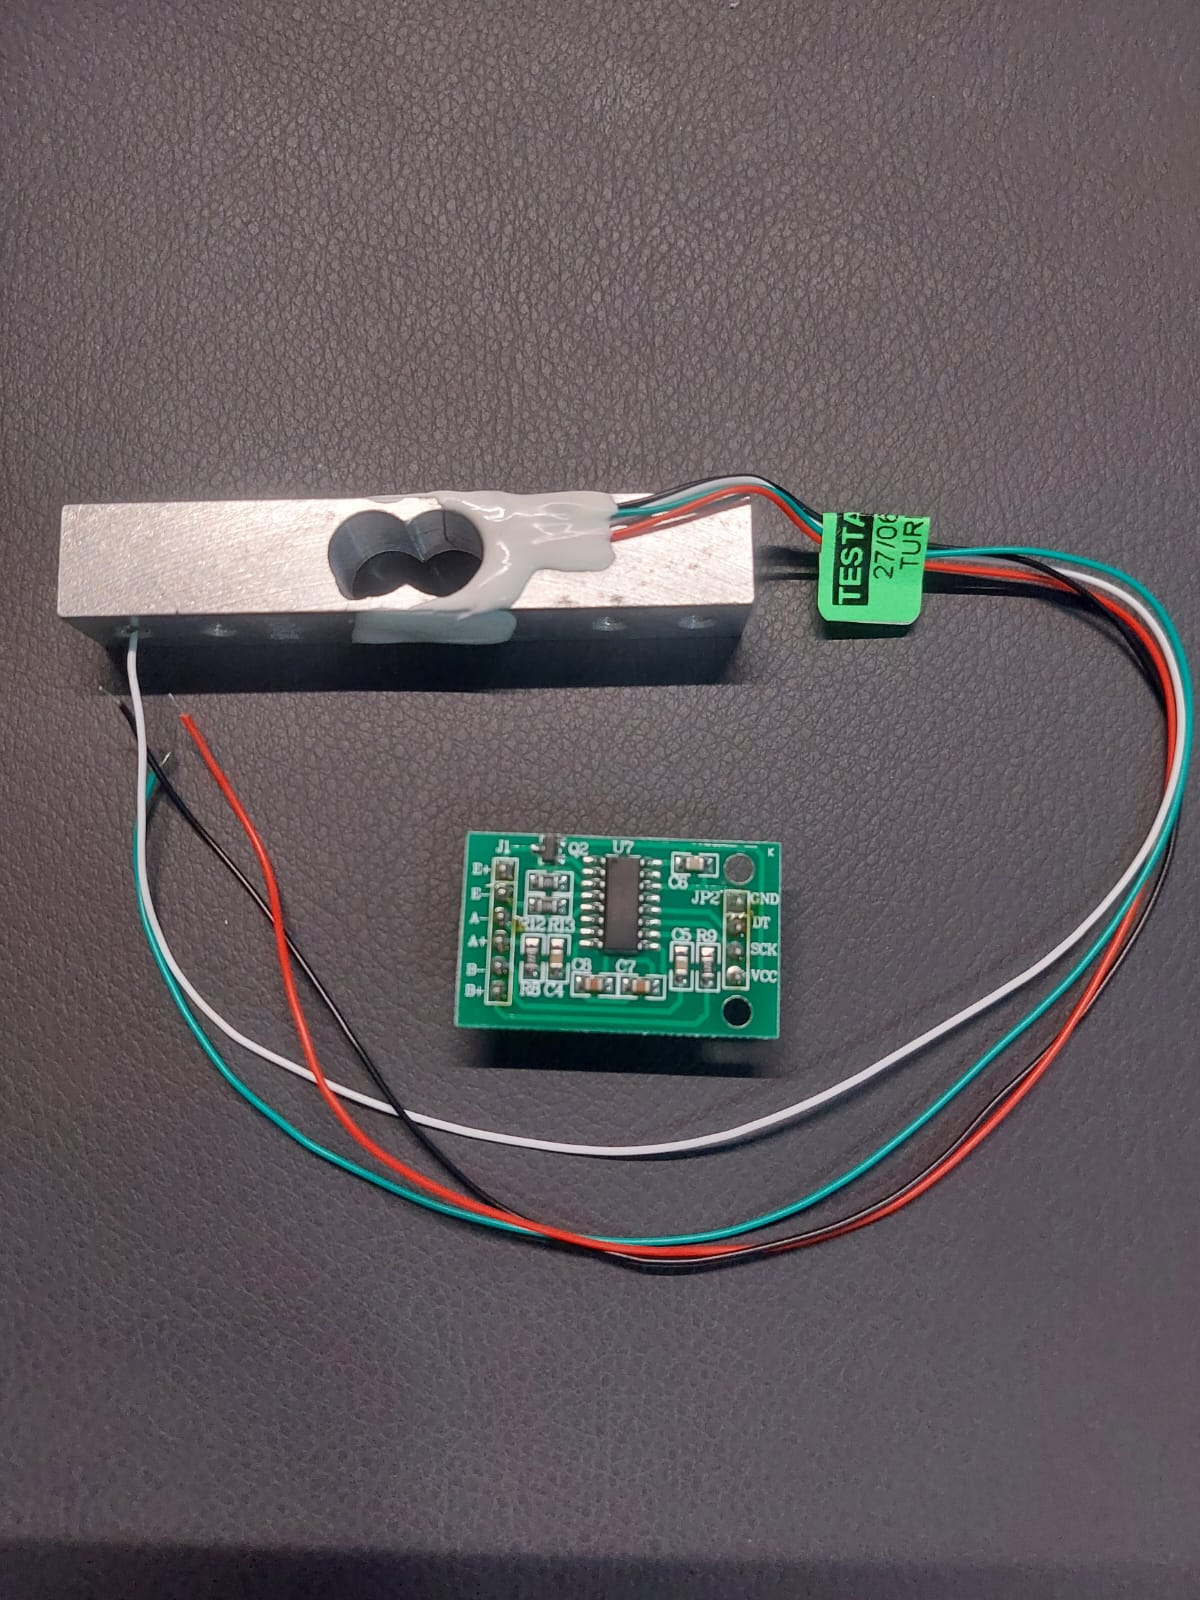
\includegraphics[width=0.4\textwidth]{./images/hx711.jpeg}
	\caption[HX711 breakout board and load cell]{HX711 breakout board and load cell}
	\fonte{}
	\label{fig:weighttesting}
\end{figure}

The HX711 integrated circuit comes in a breakout board, shown in Figure
\ref{fig:weighttesting}, that contains the necessary passive components and
includes the pin headers for connecting with other boards. The typical application 
circuit of the HX711 integrated circuit is shown in Figure \ref{fig:hx711circuit}.

\begin{figure}[H]
	\centering
	\caption[Typical HX711 circuit]{Typical HX711 circuit}
    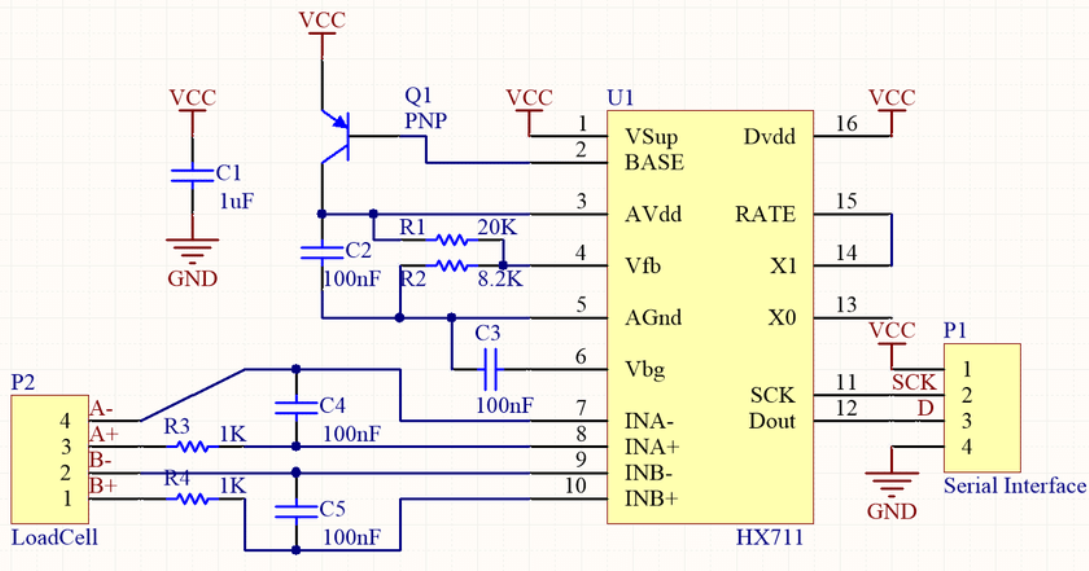
\includegraphics[width=0.8\textwidth]{./images/hx711circuit.png}
    \fonte{\cite{Ross2019}}
    \label{fig:hx711circuit}
\end{figure}

The Raspberry Pi board was connected to the HX711 through its GPIO pins,
allowing it to obtain the sensor readings through the serial interface. The
protocol used does not follow any known standard and can be
described as a \textit{Non-I2C compliant two-wire
protocol}\footnote{https://github.com/queuetue/Q2-HX711-Arduino-Library}.

An open-source driver implementation was used\footnote{https://github.com/tatobari/hx711py}, 
which included all the necessary features for the prototype.

As shown on Figure \ref{fig:devassembly}, the load cell requires a minimal
mechanical assembly to be tested properly, and for that two small wood plates
were used to secure the load cell and breakout board during development.

\begin{figure}[H]
	\centering
    \caption[Assembly used during development, including the Raspberry Pi, HX711 and load cell assembly]{Assembly used during development, including the Raspberry Pi, HX711 and load cell assembly}
    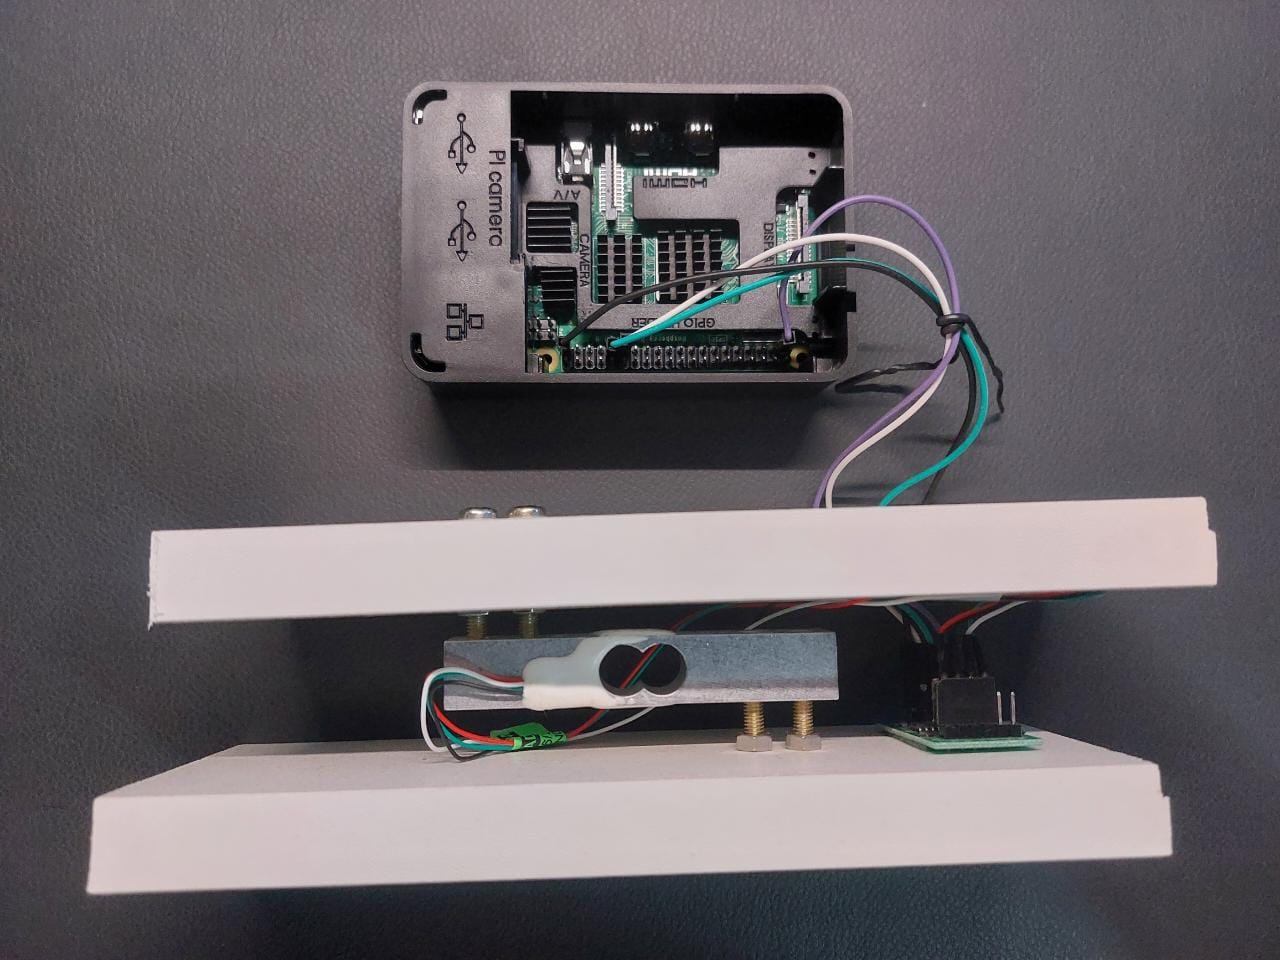
\includegraphics[width=0.7\textwidth]{./images/raspberrypiwithloadcell.jpeg}
	\fonte{}
	\label{fig:devassembly}
\end{figure}

\subsection{Camera}

In order to obtain a video feed to run object detection on, a camera system was
required. For that, a standard consumer webcam was used for its reduced cost
and good operating system driver support.

The webcam used was a Microsoft LifeCam
Cinema\footnote{https://www.microsoft.com/pt-BR/accessories/products/webcams/lifecam-cinema},
 shown in Figure \ref{fig:camera}, capable of capturing video in 720p up to 30\siglaPt{FPS}{Frames Per Second}, more
than enough for our prototyping requirements.

\begin{figure}[H]
	\centering
    \caption[Microsoft LifeCam Cinema Webcam used]{Microsoft LifeCam Cinema Webcam used}
    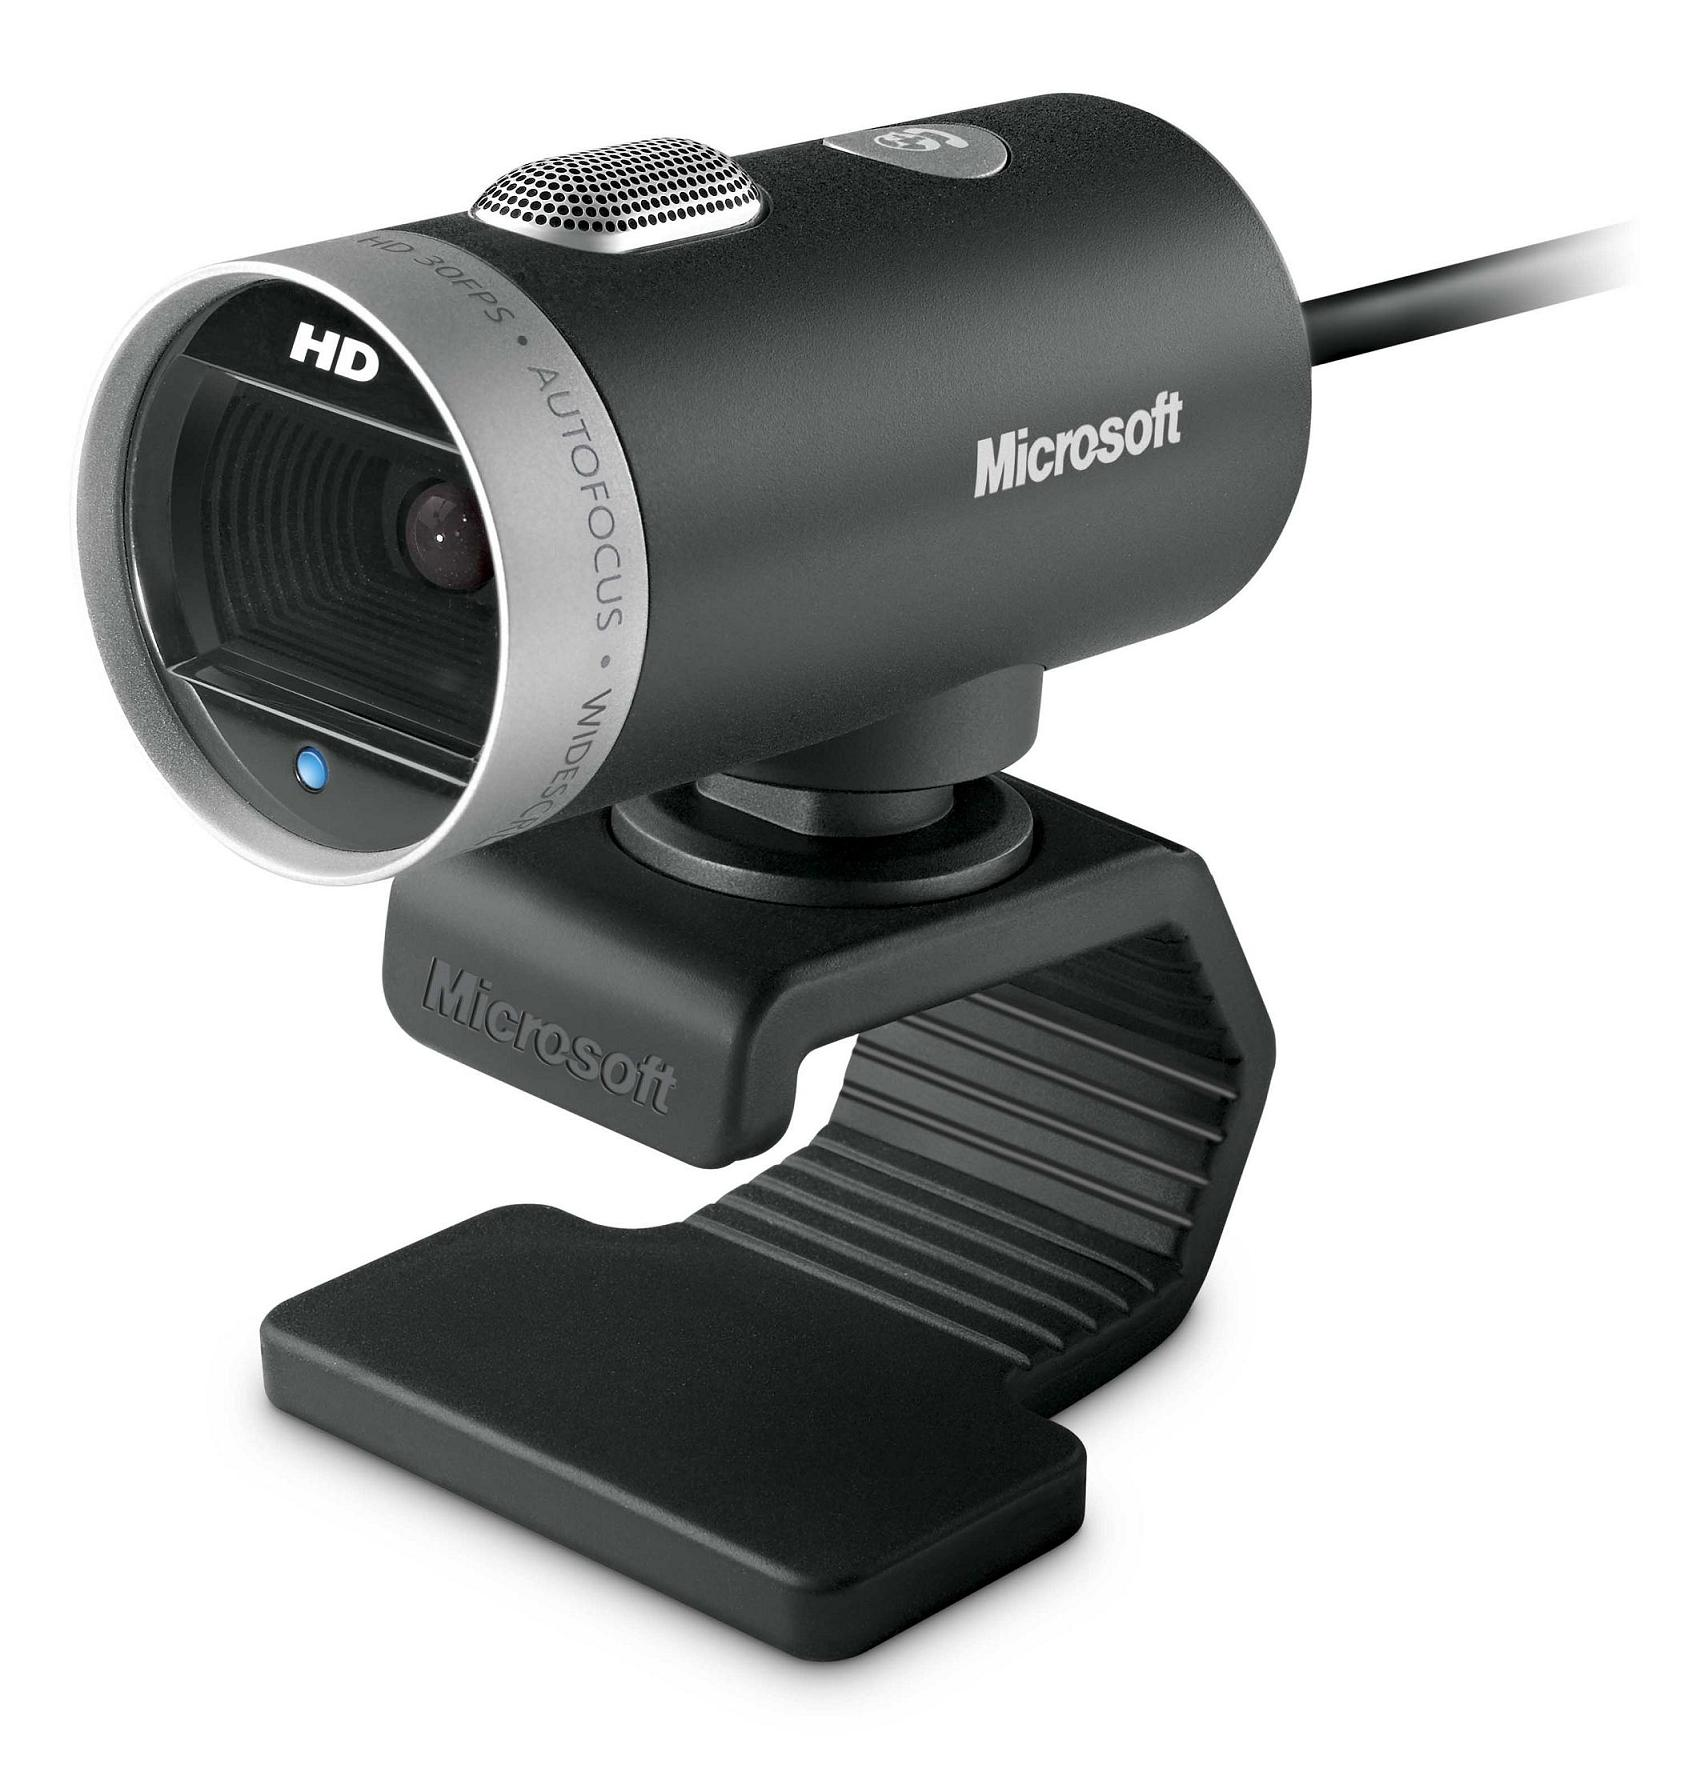
\includegraphics[width=0.3\textwidth]{./images/webcam.jpg}
	\fonte{}
    \label{fig:camera}
\end{figure}

\subsection{Application}

Developed in the Python\footnote{https://python.org} programming language, the
Product Recognizer application will provide the compute capabilities to apply
our business logic for processing the video feed provided by the camera and the
readings from the weight sensor.

The Python language was chosen for its vast tooling for working with computer
vision, sensors and interacting with the Raspberry Pi's built-in devices. The
language has also became a \textit{lingua franca} in the Machine Learning and
Data Science community as shown by volume of publications using it in the last
decade \cite{Wes2017,Joel2019,Andreas2016}.

The Product Recognizer application also uses a multi-threaded design to allow
concurrent processing, an important factor when considering the amount
\siglaPt{I/O}{Input/Output} operations performed.

Since Python's threading implementation does not allow for multiple threads to
execute in parallel -- i.e. at the same time -- a multi-process design could take
better advantage of the four available processing cores in the Raspberry Pi CPU
but that path was not explored and will be left for future iterations.

The three threads created are described below:
\begin{itemize}
    \item Frame Reader Thread: Responsible for reading frames from the Camera and making them available to the Main Thread.
    \item Main Thread: Responsible for bootstraping the application - including creating the other threads - and executing the main loop of
        object detection.
    \item Product Recognizer Thread: Responsible for applying the business logic using the objects detected and the weight sensor readings.
\end{itemize}

These threads communicate in synchronous and asynchronous means to achieve the overall goal of processing video and sensor data, as shown on Figure \ref{fig:threads}.

\begin{figure}[H]
	\centering
	\caption[Thread communication for the Product Recognizer Appplication]{Thread communication for the Product Recognizer Application}
    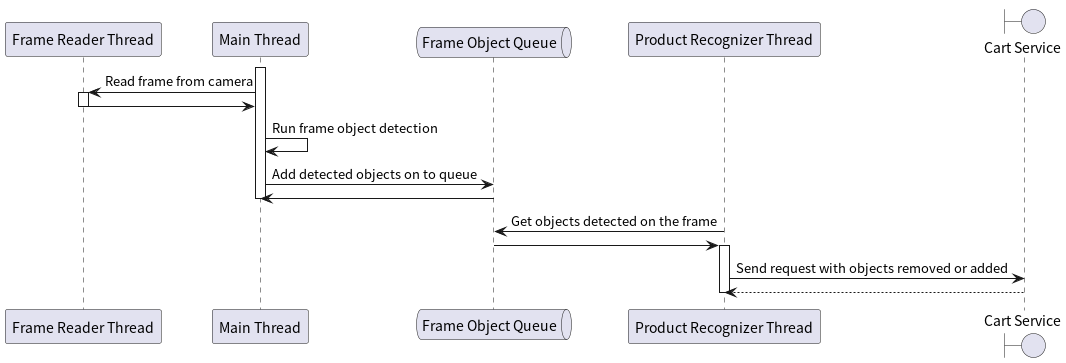
\includegraphics[width=1\textwidth]{./images/Product Recognizer Thread communication.png}
	\fonte{}
	\label{fig:threads}
\end{figure}

\begin{sourcecode}
\caption{Loop of the Main Thread. Some details were ommitted for the sake of brevity}
\begin{lstlisting}[language=Python,label={lst:main}]
while True:
  try:
    # Get frame from camera, provided by Frame Reader thread
    frame = stream.read_frame()

    # Preprocess and run object detection
    input = preprocessor.process(frame)
    detector.infer(input)

    # Filter objects by their class and confidence threshold
    objects = detector.get_objects()
    filtered_objects = object_filter.filter(objects)

    # Add filtered objects to the queue
    frame_objects_queue.put(filtered_objects)
\end{lstlisting}
\fonte{}
\end{sourcecode}

As shown on Listing \ref{lst:main} and in Figure \ref{fig:threads}, the Main
thread will do the computational work to fetch the frames from the camera that
were read by the Frame Reader thread, pre-process and run the object detection
model in it. The objects are then filtered and then added to a message queue
that will be used by the Product Recognizer thread to apply our product
detection rules.

\subsection{Product Recognizer Thread}

The Product Recognizer Thread is responsible for applying the main business
logic of detecting the addition and removal of products by leveraging the
objects detected in the frame and the readings provided by the weight sensor.

The thread will execute an infinite loop to constantly observe the objects
detected in the frame and the weight readings to detect product additions
and removals.

It uses two main variables to keep track of the current state:
\begin{itemize}
    \item A dictionary of which products are present in the cart and their count.
    \item The weight associated with the products present in the cart.
\end{itemize}

The first important step in the thread's logic is the \textit{Frame Diff}. This step 
calculates the difference in terms of the objects detected in the current 
and previous frames (e.g. whether objects were added, removed, or remain the same) 
and store it in a dictionary data structure\footnote{https://docs.python.org/3/tutorial/datastructures.html\#dictionaries},
by comparing the stored product dictionary and the received list of frame
objects from the Main Thread.

\begin{figure}[H]
	\centering
	\caption[Illustration of the frame diff'ing scheme]{Illustration of the frame diff'ing scheme. A can was added on frame $n+1$ and therefore will generate a diff of one can. If the reading from the weight sensor matches the expected one, the product will be added to the cart.}
    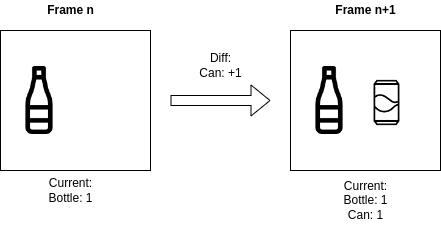
\includegraphics[width=0.8\textwidth]{./images/diagrams/framediff.png}
	\fonte{}
    \label{fig:diff}
\end{figure}

Given the frame object diff, it is then possible to calculate an expected
weight change based on the weight of each item - and their quantity - contained
in the diff. The expected weight difference is then compared to the actual
one obtained from the weight sensor, considering a configurable tolerance.

In this scenario, the weight readings are used as a filter and act as a
\textit{commit} step for differences detected in the frame objects. This way, objects are not
added or removed from the cart simply by appearing or disappearing from the frame.

In the example show in Figure \ref{fig:diff}, if the illustrated can weights an expected 400 grams, the weight
difference expected should be close to 400 grams. If the weight difference does not match the expected
one, the object will not be considered for addition or removal. 

A more detailed activity diagram of the logic executed in the Product Recognizer thread loop is
shown in Figure \ref{fig:activity}.

\begin{figure}[H]
	\centering
	\caption[Activity diagram for the Product Recognizer thread]{Activity diagram for the Product Recognizer thread}
    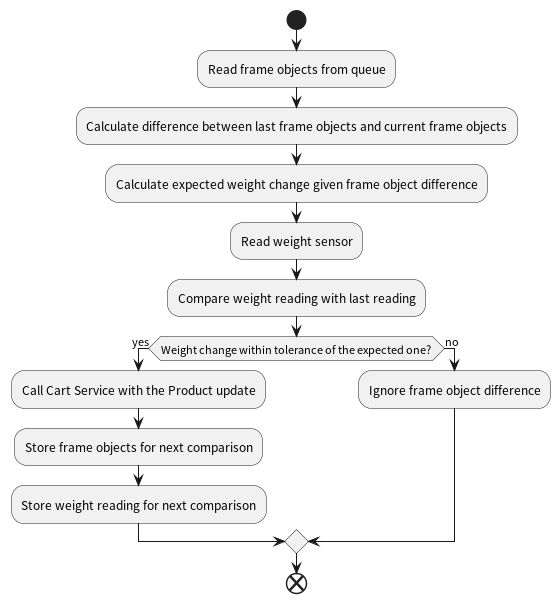
\includegraphics[width=0.8\textwidth]{./images/Product Recognizer Activity.png}
	\fonte{}
    \label{fig:activity}
\end{figure}

\begin{sourcecode}
\caption{Product Recognizer thread logic}
\begin{lstlisting}[language=Python]
objects = self.queue.get_nowait()

# Preprocessing step just to format data
current_frame_objects = self.__build_object_dict(objects)

# Calculate the frame diff using the last and current frame objects
frame_diff = self.__get_frame_diff(
    current_frame_objects, self.last_frame_objects
)

if len(frame_diff) == 0:
    self.log.info("empty diff")
    continue

# Get current weight reading
weight_reading = self.weight_sensor.get_reading(samples=5)

for label, count in frame_diff.items():
    if not self.__valid_weight_difference(label, count, weight_reading):
        self.log.info("ignoring, not valid weight difference")
        continue

    # Send request to cart service
    self.__call_cart_service(label, count)

    # Update stored state
    self.last_weight_reading = weight_reading
    self.last_frame_objects[label] = current_frame_objects[label]
    if self.last_frame_objects[label] == 0:
        del self.last_frame_objects[label]
\end{lstlisting}
\fonte{}
\end{sourcecode}

\subsection{Object Detection Model}

The code used to train our Object Detection models was made available in GitHub,
in our Project's Repository
\footnote{https://github.com/fsmiamoto/zcart/blob/master/product\_recognizer/model/notebooks/}.
It can be used for reference and for performing a further deep dive into this section.

Five products were chosen for the purpose of setting up and demonstrating the Object Recognition 
capability of our product: a Blue Pens Packet; a Card Deck; a Coke Can; a Guarana Soda Can; 
and a Post It Pack. 
The data used for training our custom Object Detection model was collected and labelled by us
using Edge Impulse\footnote{https://www.edgeimpulse.com/}, a development platform for Machine 
Learning on Edge devices.
A total of \textbf{1000 photos} were taken using the Data Collection feature of
the Edge Impulse Studio, shown in Figure \ref{fig:edgeimpulse1}, using the same
webcam that is used for the inference in our final product. Our photos included
images showing each one of the products in different scenarios and positions,
and also images where more than one product was present.

\begin{figure}[H]
	\centering
	\caption[Collecting Data in Edge Impulse]{Collecting Data in Edge Impulse}
    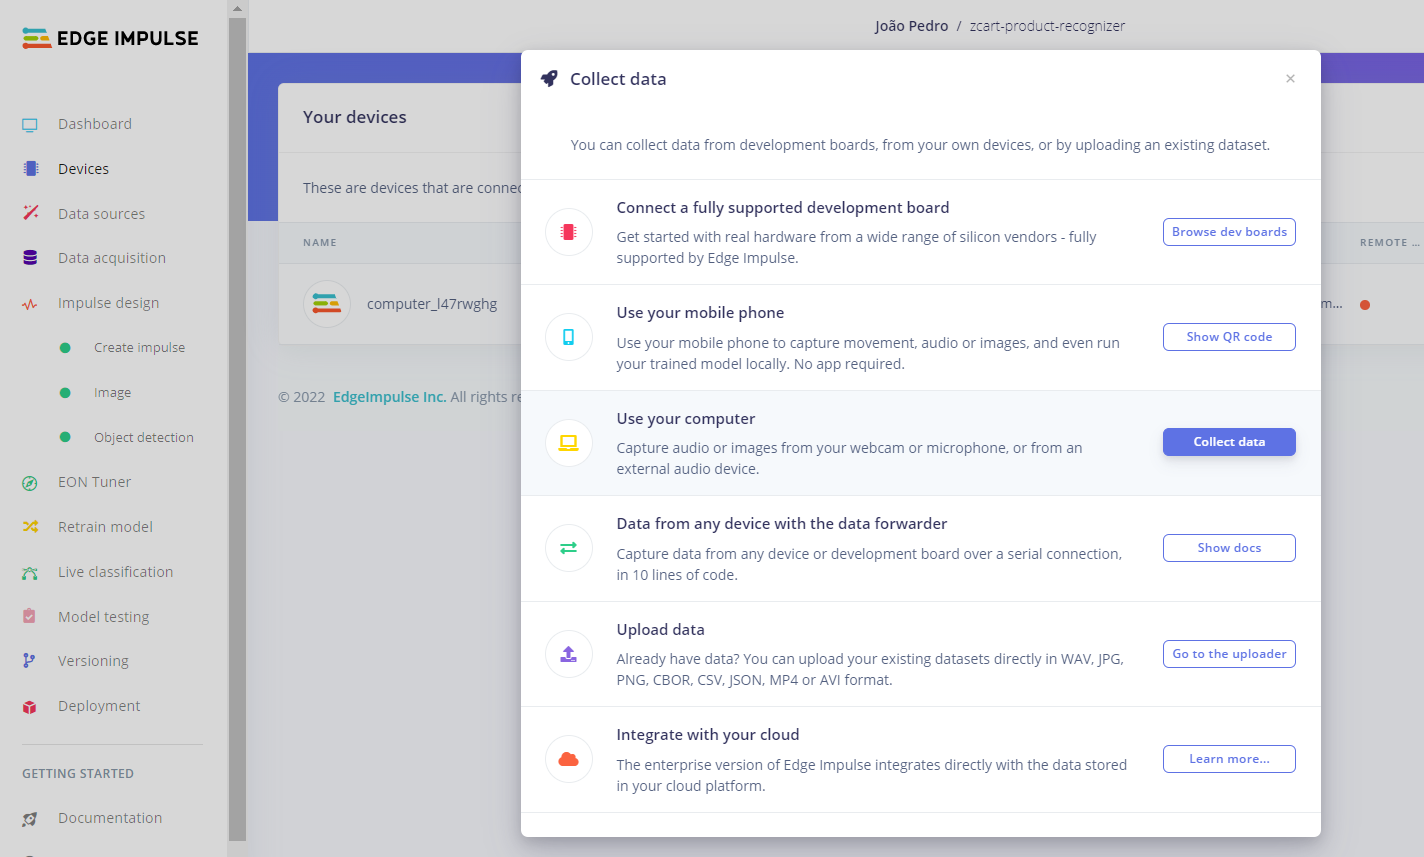
\includegraphics[width=0.8\textwidth]{./images/edge-impulse-collect-data.png}
	\fonte{Edge Impulse (2022)}
    \label{fig:edgeimpulse1}
\end{figure}

The pictures were then were labeled using the Labeling
Queue\footnote{https://docs.edgeimpulse.com/docs/edge-impulse-studio/data-acquisition/labeling-queue}
feature of Edge Impulse, which allowed us to draw Bounding Boxes around the
desired objects for detection, as shown in Figure \ref{fig:edgeimpulse2}.

\begin{figure}[H]
	\centering
	\caption[Labelling Queue in Edge Impulse]{Labeling Queue in Edge Impulse}
    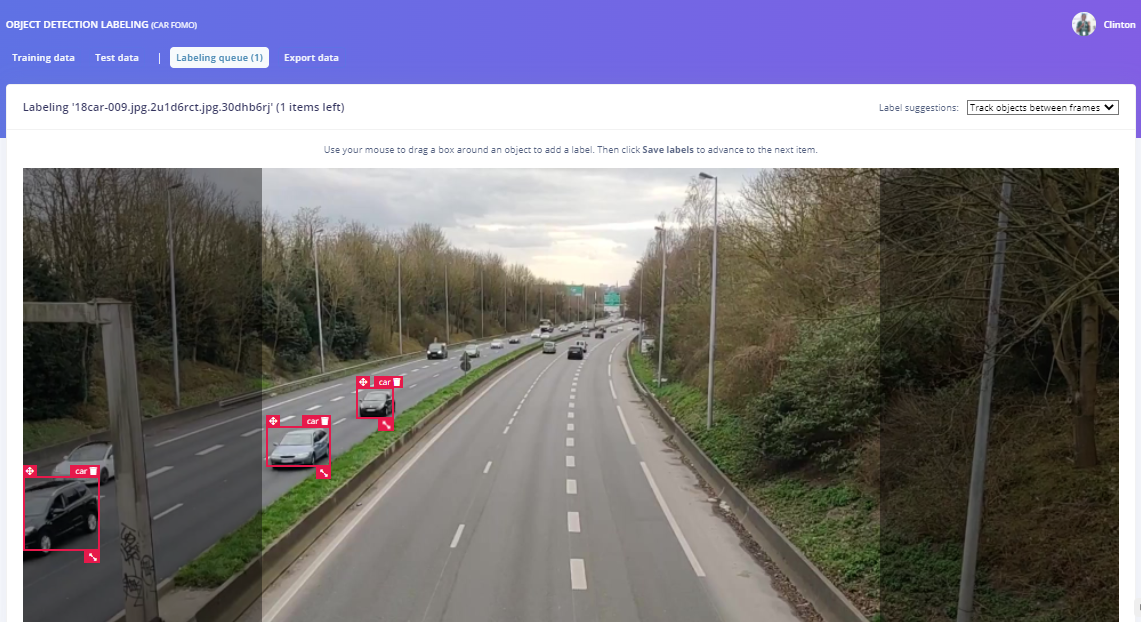
\includegraphics[width=0.9\textwidth]{./images/edge-impulse-labelling-queue.png}
	\fonte{Edge Impulse (2022)}
    \label{fig:edgeimpulse2}
\end{figure}

The raw pictures and bounding boxes were then exported from Edge Impulse such
that we could pre-process the data and model our custom object detection
algorithm using the Python programming language. The pictures were exported in
their raw JPEG\footnote{Defined in ISO/IEC 10918}  file format, comprised in a
ZIP folder. The bounding boxes were exported in the format of a JSON file
containing the coordinates for the boundaries and the metrics for each picture,
allowing us to easily reconstruct the bounding boxes for each object in each
image using programming instructions. The files were then loaded to a Cloud
Object Storage Bucket in AWS \footnote{https://aws.amazon.com/}, making it
easier for us to access the data by importing it from the web using any
programming language.

Listing \ref{lst:boundingBoxCoordinates} shows a section of an example JSON file containing
the bounding boxes.

\begin{sourcecode}
\caption{Bounding boxes coordinates file exported from Edge Impulse}
\begin{lstlisting}[label={lst:boundingBoxCoordinates}]
	{
		"version": 1,
		"type": "bounding-box-labels",
		"boundingBoxes": {
		  "im1.jpg": [
			{
			  "label": "blue_pens",
			  "x": 120,
			  "y": 265,
			  "width": 172,
			  "height": 207
			},
			{
			  "label": "card_deck",
			  "x": 285,
			  "y": 120,
			  "width": 136,
			  "height": 247
			}
		  ],
		  "im2.jpg": [
			(...)
		  ]
		}
	}
\end{lstlisting}
\fonte{}
\end{sourcecode}

The development environment used for writing the code for training our custom
model was Google Colab\footnote{https://colab.research.google.com/}, and the
programming language of choice was Python. Google Colab consists on a web-based
interface, shown in Figure \ref{fig:googlecollab}, that allows developers to
use Google's infrastructure (with GPUs and TPUs) for writing and executing
code.

\begin{figure}[H]
	\centering
	\caption[Google Colab - Overview of Colaboratory Features]{Google Colab - Overview of Colaboratory Features}
    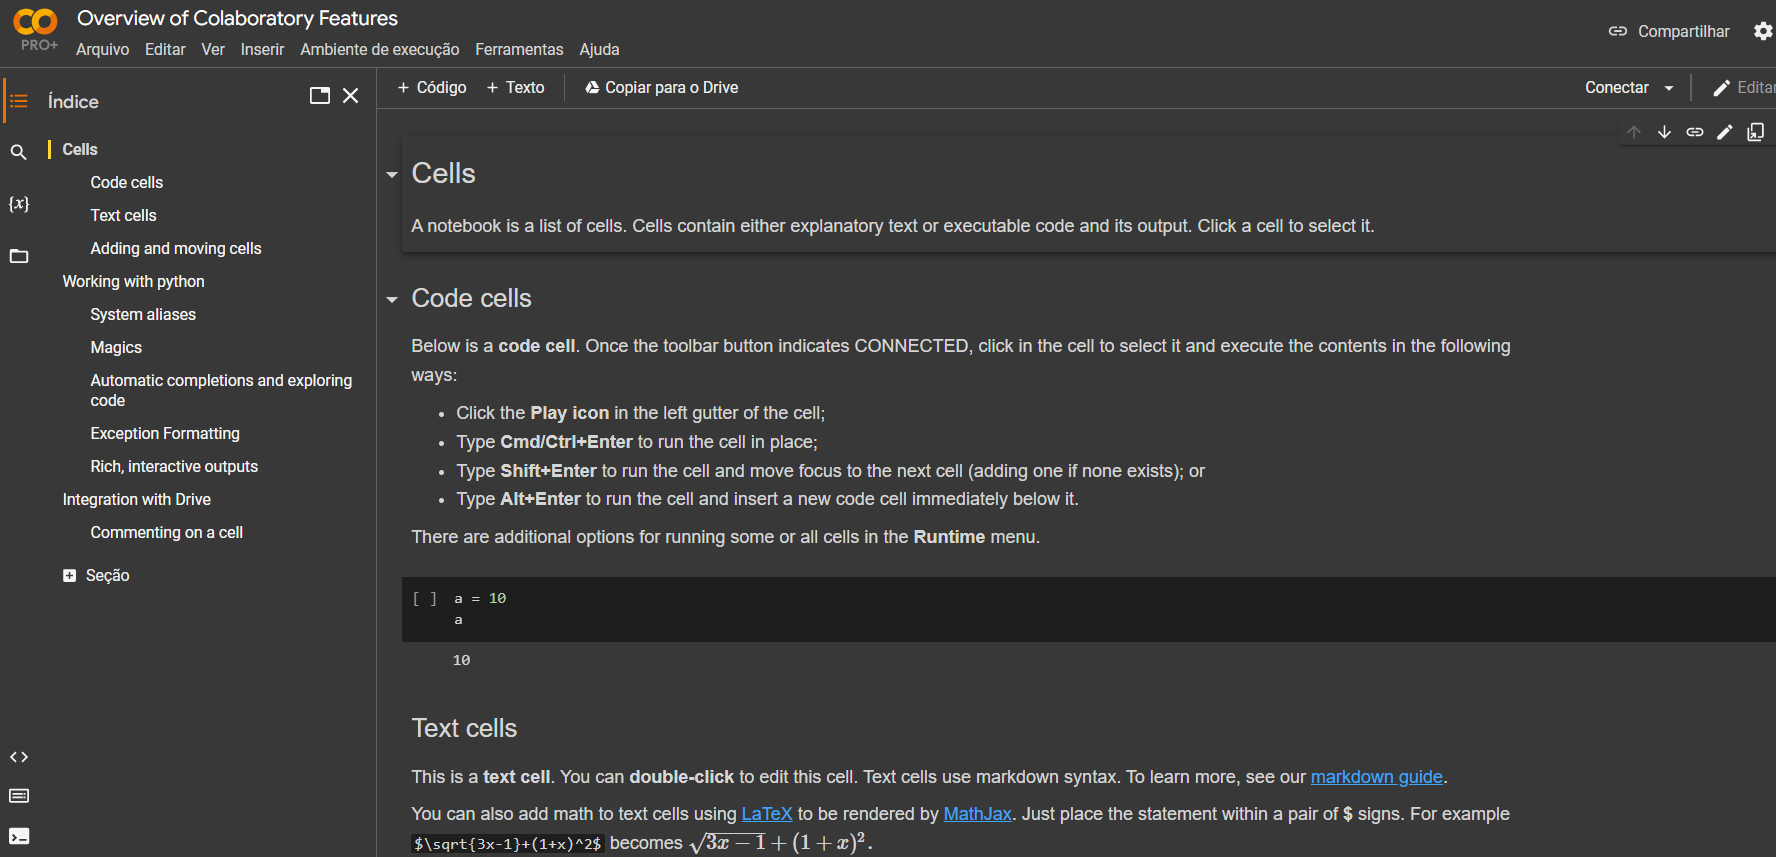
\includegraphics[width=1\textwidth]{./images/google-colab.png}
	\fonte{Google\footnote{https://colab.research.google.com/notebooks/basic\_features\_overview.ipynb}}
    \label{fig:googlecollab}
\end{figure}

The Edge Impulse files were loaded from our cloud object storage bucket, and then manipulated in Python
from Google Collab such that we could utilize the images and bounding box coordinates for training
our model.

We decided to use Google's TensorFlow\footnote{https://www.tensorflow.org/} framework to train our 
models, as it is one of the most popular frameworks employed in the Industry for training AI models
and also because it features a lightweight library called TensorFlow Lite\footnote{https://www.tensorflow.org/lite}, 
which is appropriate for creating efficient edge and mobile AI models considering the 
typical hardware constraints from these types of devices.

To train our model, we used the TensorFlow Lite's ModelMaker API\footnote{https://www.tensorflow.org/lite/models/modify/model\_maker} 
for Object Detection, which simplifies the process of training our models by breaking down the most
complex concepts of deep learning into parameterized objects and methods, allowing us to spend
more time on the pre-processing steps and on experimenting with different network configurations
to improve the model's accuracy. 

As of writing this work, the ModelMaker API only has compatibility
with the EfficientDet family of architectures \cite{Mingxing2020} for training
Deep Learning models for Object Detection. The EfficientDet family is efficient
for object recognition in edge devices, altough contemporany architectures,
such as the YOLOv5 and its successors, can have better performance, as shown in Figure \ref{fig:yoloefficientdet}.

\begin{figure}[H]
	\centering
	\caption[YOLOv5 vs EfficientDet - Performance Comparison]{YOLOv5 vs EfficientDet - Performance Comparison}
    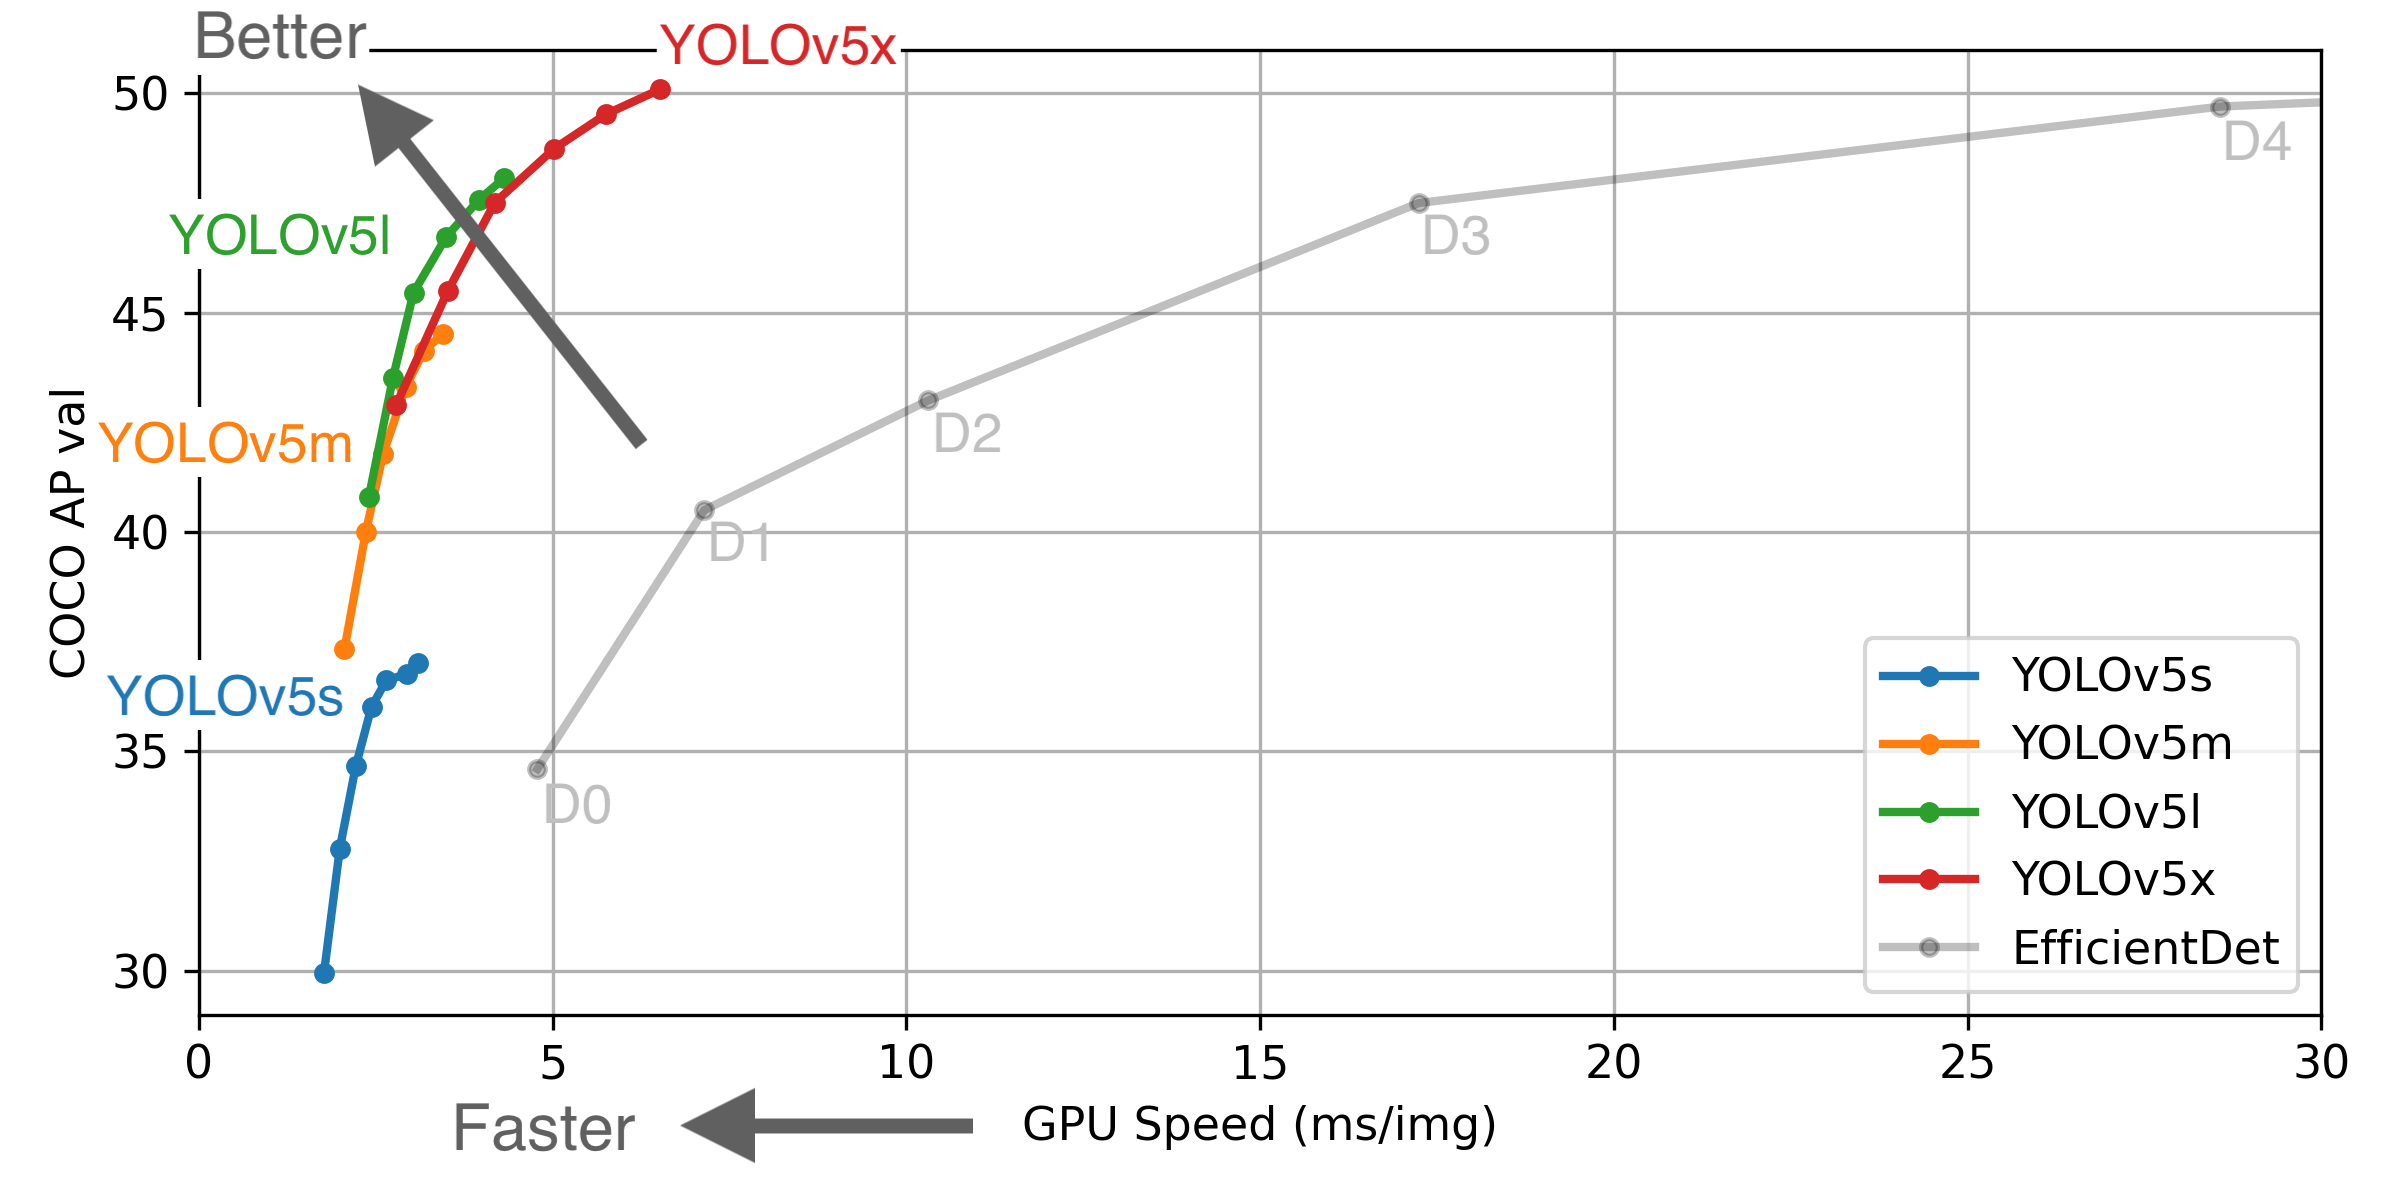
\includegraphics[width=0.9\textwidth]{./images/yolo-efficientdet-comparison.png}
	\fonte{YOLOv5 Release Notes\footnote{https://github.com/ultralytics/yolov5/releases/tag/v4.0}}
    \label{fig:yoloefficientdet}
\end{figure}

Our initial plan was to use the YOLOv5 architecture, but since its
implementation is not native to TensorFlow Lite, it would require us to create
additional wrappers around the outputs of the YOLOv5 network to get it working
as expected. Even thought it is possible to convert the models from their
original PyTorch\footnote{https://pytorch.org/} format to a TensorFlow Lite
format, the conversion does not cover some of the features from the original
implementation\footnote{https://github.com/ultralytics/yolov5/issues/1981},
which limits its direct functionality. Similar compatibility issues happen with
the latest YOLO implementations, such as the
YOLOv7\footnote{https://medium.com/geekculture/journey-putting-yolo-v7-model-into-tensorflow-lite-object-detection-api-model-running-on-android-e3f746a02fc4}.
Thus, we have decided to proceed with the TensorFlow Lite's Model Maker API
compatible architectures -- namely the EfficientDet family --  since it would
have taken a considerable time to troubleshoot conversion defects from the YOLO
architecture and all that work would not bring any additional value to our
prototype.

Since our original images were saved in the 640x480 resolution and the expected
input of the EfficientDet network is of 320x320 px, two pre-processing
approaches were tried out for the training dataset: resizing and cropping the
images. The bounding box coordinates and dimensions were also adjusted
accordingly such that the data integrity was preserved. Figure
\ref{fig:preprocess} illustrates both of the approaches used.

\begin{figure}[H]
	\centering
	\caption[Image Preprocessing Strategies]{Image Preprocessing Strategies}
    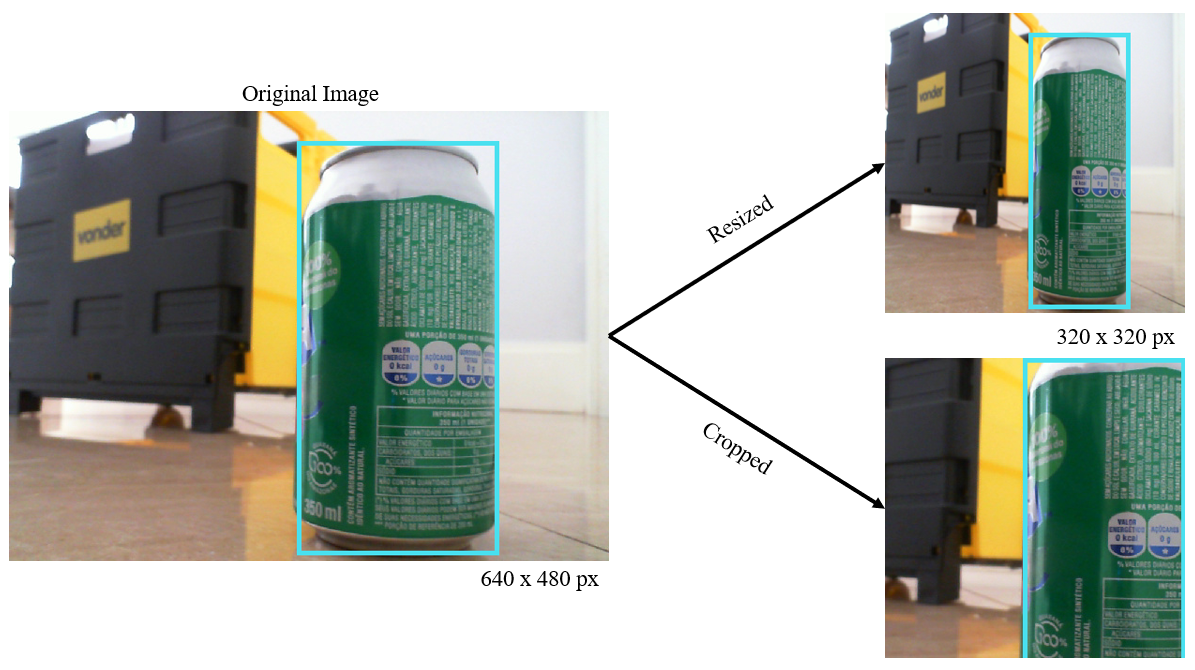
\includegraphics[width=1\textwidth]{./images/image_preprocessing.png}
	\fonte{}
    \label{fig:preprocess}
\end{figure}

Once the images and bounding boxes were pre-processed, the images were split
into Train, Validation and Test sets; and saved in the standardized format
required by the TensorFlow Lite's Model Maker for Object Detection API for
training, which consists of a Comma Separated Values (\siglaPt{CSV}{Comma
Separated Values}) file with the structure shown in Listing \ref{lst:csvFormatTrain}.

\begin{sourcecode}
\caption{CSV format for specifying the Train, Test and Validation 
	image sets for training models using the TensorFlow's Model Maker API for Object 
	Detection}
\begin{lstlisting}[label={lst:csvFormatTrain}]
Template:
set,path,label,x_min,y_min,,,x_max,y_max,,
set,path,label,x_min,y_min,x_max,y_min,x_max,y_max,x_min,y_max

Examples:
TEST,./images_path/im3.png,0.5,0.6,,,0.2,0.9,,
VALIDATION,./images_path/im4.png,coke_soda,0.3,0.4,,,0.4,0.8,,
TRAIN,./images_path/im5.png,guarana_soda,0.3,0.3,0.8,0.8,1.0,0.9,0.1,1.0
TRAIN,./images_path/im5.png,post_it,0.3,0.1,,,0.3,0.4,,
\end{lstlisting}
\fonte{}
\end{sourcecode}

Approximately 70\% of the photos shot were moved to the Train set, which is the set used for effectively 
tuning the weights and biases of the custom models; About 21\% were moved to the Validation set, 
being used to understand our model's performance under different training scenarios and steps; 
and the rest was used for testing the custom model after it was trained, which allowed us to 
get unbiased metrics on how it would approximately perform in real life \cite{MluExplain}.

Table \ref{tbl:imageSetsTab} describes the data sets created for training and evaluation in greater detail.

\begin{table}[H]
	\centering
	\caption[Image Sets Created for Training, Validation and Testing]{Image Sets Created for Training, Validation and Testing}
	\begin{adjustbox}{width=1\textwidth}
	\label{tab:imageSets}
	\begin{tabular}{c|c|c|c|c}
		\hline 
		Class & Number of Pictures & Pictures in the Train Set & Pictures in the Validation Set & Pictures in the Test Set \\
		\hline
        Blue Pens Packet & 293 & 206 & 61 & 26\\
		Card Deck & 306 & 215 & 64 & 27\\
		Coke Can & 276 & 194 & 58 & 24\\
		Guarana Soda Can & 283 & 199 & 59 & 25\\
		Post It Pack & 273 & 192 & 57 & 24\\
		\hline 
	\end{tabular}
	\end{adjustbox}
	\label{tbl:imageSetsTab}
	\fonte{}
\end{table}

Finally, we defined a programming loop to train different models using the EfficientDet-D0,
EfficientDet-D1, EfficientDet-D2, EfficientDet-D3 and EfficientDet-D4 architectures; both by
applying Transfer Learning on the top of pre-trained weights from training with the COCO-2017 dataset 
\footnote{https://cocodataset.org/\#home} and by training the entire networks based in our custom data. 

We ran this entire loop using the cropped images first; and then executed it using resized images with the EfficientDet-D0,
EfficientDet-D1 and EfficientDet-D2 architectures too, as they were the ones who offered better
performance balance considering our hardware constraints. 
With that, we came to have 16 distinct custom models for experimenting, as shown in Table \ref{tbl:modelsTrainedTab}.

\begin{table}[H]
	\centering
	\caption[Models Trained]{Models Trained}
	\begin{adjustbox}{width=1\textwidth}
	\label{tab:modelsTrained}
	\begin{tabular}{c|c|c|c}
		\hline 
		Model & Image Pre-Processing Strategy & Architecture & Whole Trained/Transfer Learning \\
		\hline
        1 & Cropping & EfficientDet-D0 & Whole Trained \\
		2 & Cropping & EfficientDet-D1 & Whole Trained \\
		3 & Cropping & EfficientDet-D2 & Whole Trained \\
		4 & Cropping & EfficientDet-D3 & Whole Trained \\
		5 & Cropping & EfficientDet-D4 & Whole Trained \\
		6 & Cropping & EfficientDet-D0 & Transfer Learning on COCO-2017 \\
		7 & Cropping & EfficientDet-D1 & Transfer Learning on COCO-2017 \\
		8 & Cropping & EfficientDet-D2 & Transfer Learning on COCO-2017 \\
		9 & Cropping & EfficientDet-D3 & Transfer Learning on COCO-2017 \\
		10 & Cropping & EfficientDet-D4 & Transfer Learning on COCO-2017 \\
		11 & Cropping & EfficientDet-D0 & Whole Trained \\
		12 & Cropping & EfficientDet-D1 & Whole Trained \\
		13 & Resizing & EfficientDet-D2 & Whole Trained \\
		14 & Resizing & EfficientDet-D0 & Transfer Learning on COCO-2017 \\
		15 & Resizing & EfficientDet-D1 & Transfer Learning on COCO-2017 \\
		16 & Resizing & EfficientDet-D2 & Transfer Learning on COCO-2017 \\
		\hline 
	\end{tabular}
	\end{adjustbox}
	\label{tbl:modelsTrainedTab}
	\fonte{}
\end{table}

\section{Mechanical Assembly}

A foldable utility cart was selected as a core
component with two additional wood plates, used for creating a \textit{false
bottom} shown in Figure \ref{fig:falsebottom}. Between the plates, the load cell and Raspberry Pi board were secured
in place using bolts, screws and velcro.

Figures \ref{fig:prototype1} and \ref{fig:prototype2} show an overview of the structure built.

\begin{figure}[H]
	\centering
	\caption[Overall mechanical assembly including the LCD and Camera]{Overall mechanical assembly including the LCD and Camera}
    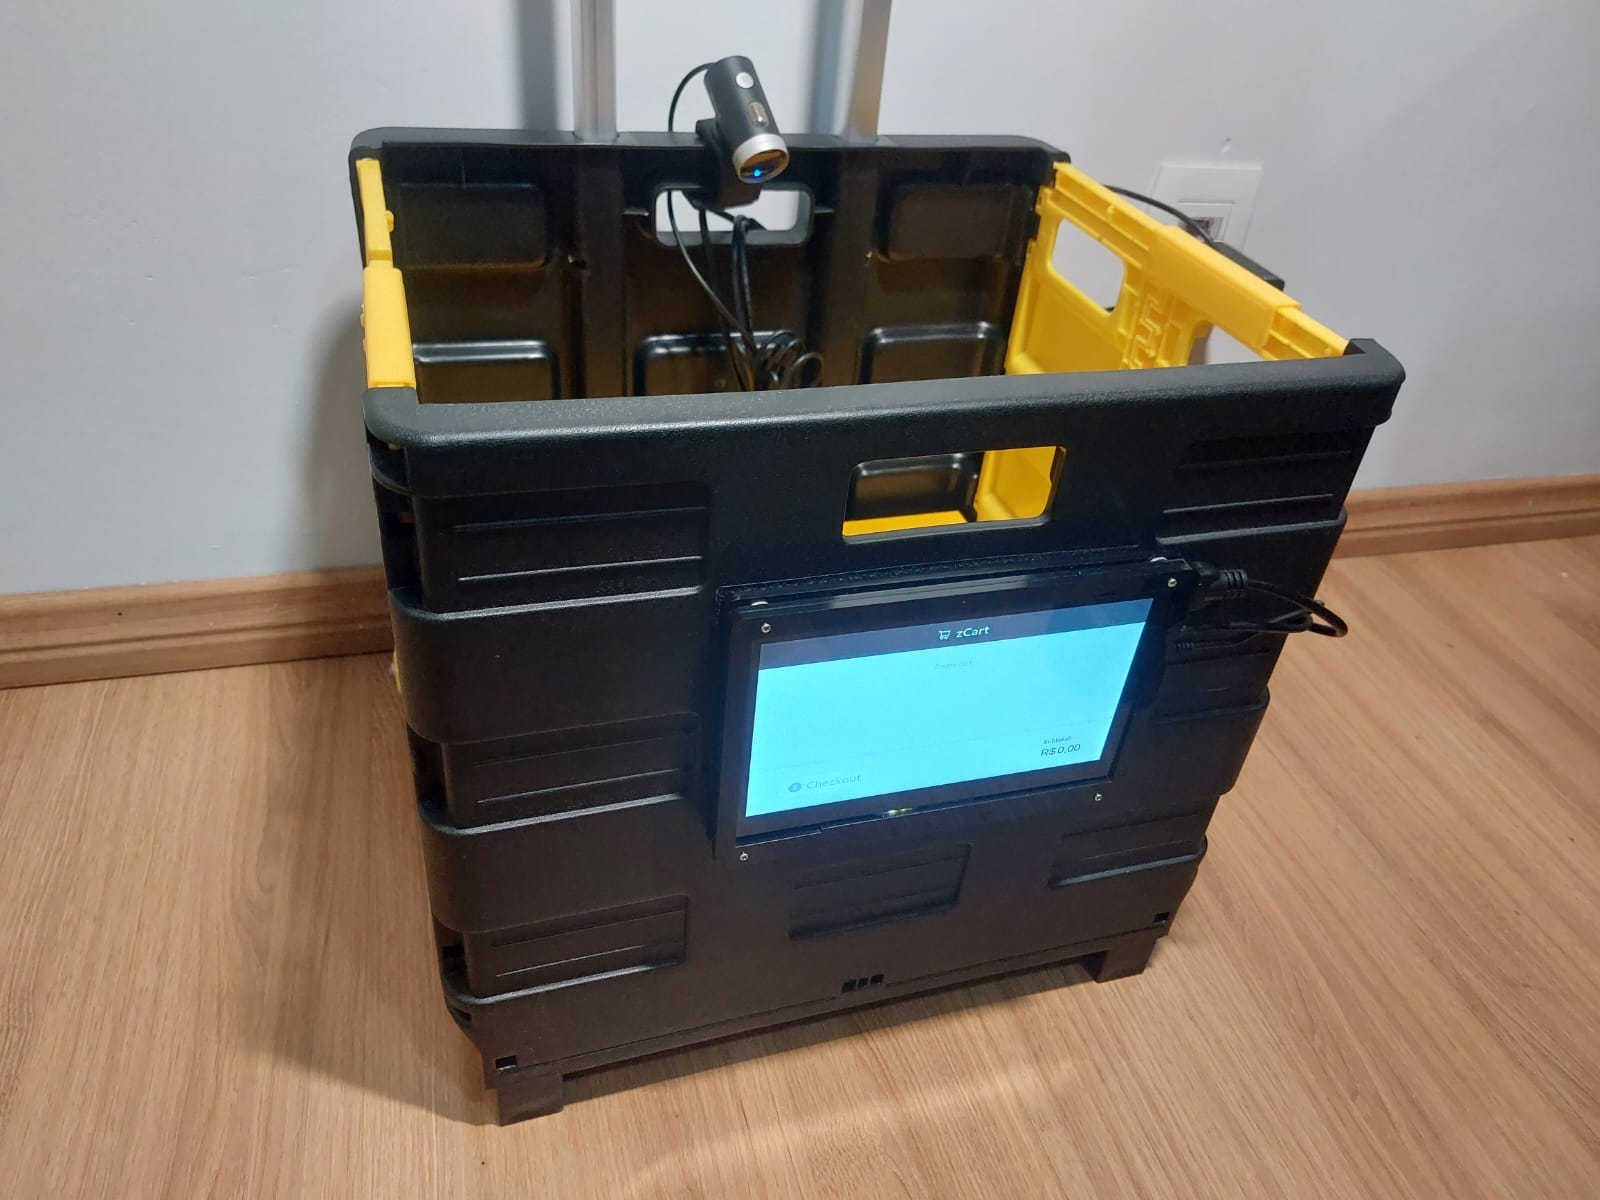
\includegraphics[width=0.75\textwidth]{./images/cart.jpeg}
	\fonte{}
    \label{fig:prototype1}
\end{figure}

\begin{figure}[H]
	\centering
	\caption[Top view of the assembly showing the false bottom]{Top view of the assembly showing the false bottom}
    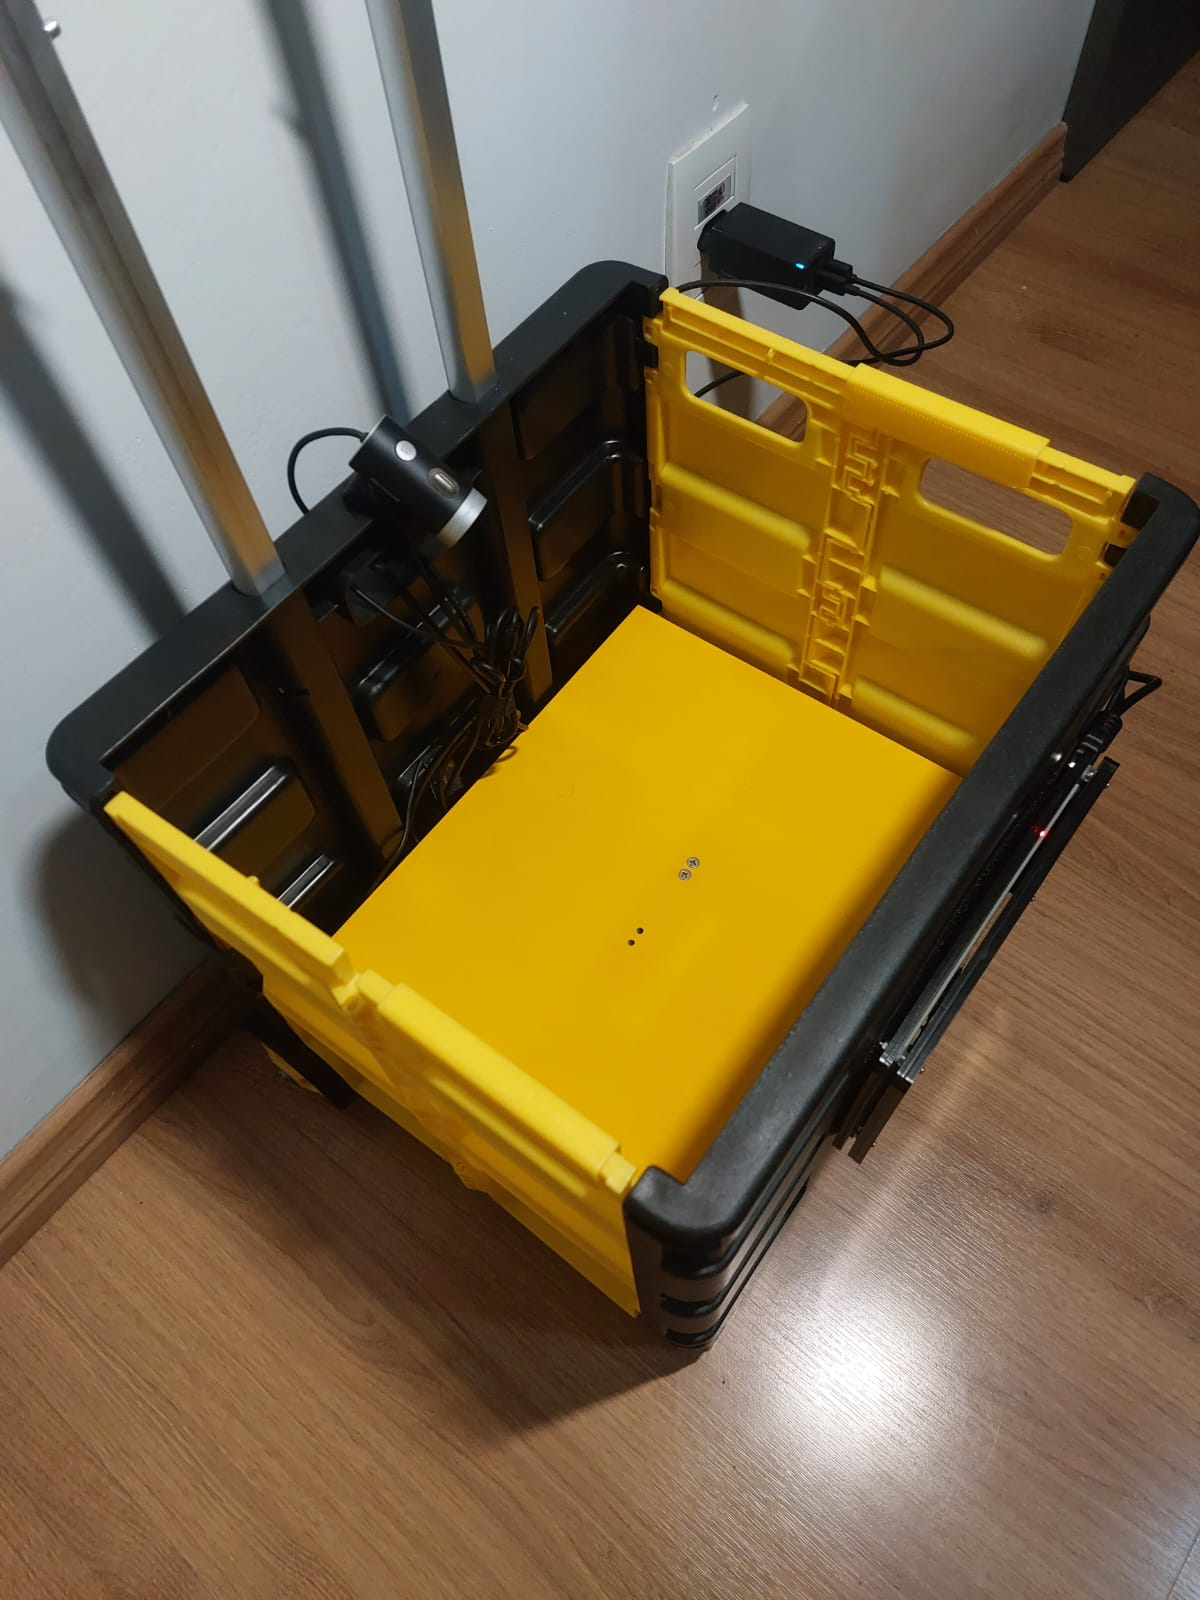
\includegraphics[width=0.5\textwidth]{./images/carttop.jpeg}
	\fonte{}
    \label{fig:prototype2}
\end{figure}

Considering the objectives of the prototype, the shape of the mechanical
housing was not considered to be of great relevance and using a real
supermarket cart would have been impractical considering its size and cost. Still, we wanted
to keep a shape that would represent the overall idea of a smart cart.

\begin{figure}[H]
	\centering
	\caption[False bottom structure with the load cell and Raspberry Pi board in between]{False bottom structure with the load cell and Raspberry Pi board in between}
    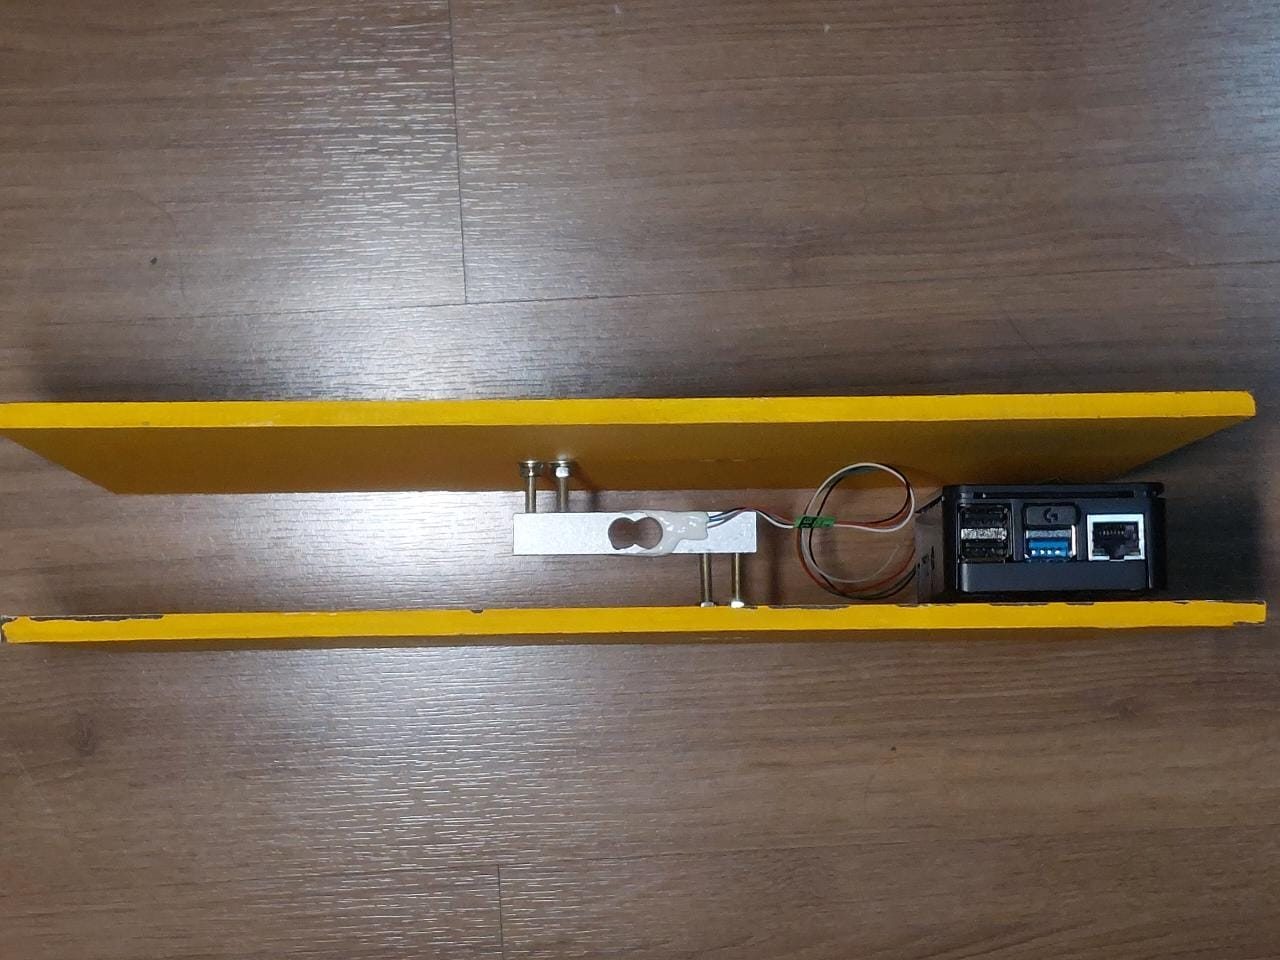
\includegraphics[width=0.6\textwidth]{./images/cartbase2.jpeg}
	\fonte{}
    \label{fig:falsebottom}
\end{figure}

Additional photos of the prototype can be seen on Appendix \ref{app:photos}.
